\documentclass[../report.tex]{subfiles}
\begin{document}	
\chapter{Experiments}
% How much do i discuss the results - You show the results and interpret the results with the reader

	\section{Unit tests}
	To analyze the design various tests are performed. The strategy followed resembles similarity to unit tests where each of the components are tested and verified to understand the design. Also, the results are normalized to analyze the performance of \gls{mems} \gls{tpr}. 
	
	\noindent The test cases followed during the fabrication process are discussed below. 
	\begin{itemize}[leftmargin=*]
		\item[$\square$] \textbf{Dose test:} The first test requires to verify the dose of \gls{hsq} and \gls{zep} used in masking to prevent the damage of masked Si. For this different doses are applied on different portion of the chip by using similar CAD model.
		
		\item[$\square$] \textbf{TE/TM\textemdash TE/TM grating with a normal waveguide:} To check any optical design it is necessary to couple the light into the chip with good transmission. That is why gratings are necessary. To check \gls{pr} design, it was necessary first to check the \gls{te} and \gls{tm} transmissions. Hence, the first test case was to check the \gls{te}/\gls{tm} grating with a normal waveguide. This give an idea of transmission parameters and the next results were referenced to this value. This test ensured that the gratings worked as intended. 
		
		\item[$\square$] \textbf{TE/TM\textemdash TE/TM grating with tapers:} The next test was to check the transmission parameters of the tapers, which was obtained by just putting the tapers end-to-end after the gratings from both ends. In this test it was made sure that the \gls{te} and \gls{tm} modes were guided through the tapers.
		
		\item[$\square$] \textbf{TE/TM\textemdash TM/TE grating with taper, normal waveguide and PBS:} Next it was necessary to check the \gls{pbs} design based on asymmetrical directional coupler, required for the characterization of the converted modes. This test ensures that both \gls{te} and \gls{tm} mode can be guided to the respective ports and the \gls{per} can be measured.
		
		\item[$\square$] \textbf{TE/TM\textemdash TE/TM grating with taper and thinner waveguide:} Since, the \gls{pr} was on a thinner waveguide of thickness \SI{230}{\nano \meter} whereas the gratings had a thickness of \SI{12}{\micro \meter}, it was necessary to use tapers to connect the gratings to the \gls{pr} section. But before checking the \gls{pr}, it was necessary to check if the transmission in a normal waveguide without the \gls{pr}. That is why this test was performed. 
		
		\item[$\square$] \textbf{TE/TM grating with PR and PBS:} Now that all the auxiliary components have been tested, the \gls{pr} design was tested as well with \gls{pbs} and \gls{te}/\gls{tm} grating for different lengths with taper.
		
		\item[$\square$] \textbf{Cantilever actuation with separation strategy:} Since, the actuation is done by applying a voltage it is necessary to check that the cantilever actuates properly on applying voltage and does not stick after removal of voltage. This is done by segregating the cantilever portion from other parts of the chip so that other portions of the chip are not affected. 
		
		\item[$\square$] \textbf{TE/TM Grating with PR, PBS, MEMS waveguide and actuation:} Finally, if all the previous tests have succeeded, the final design is tested with all the components and characterized.
	\end{itemize}
	
	\noindent The goal of the unit test strategy was to find and understand any short-comings which might occur at any stage of the fabricated process.
	
	\section{Characterization}
	An optical test bench setup was used to characterize the product. The test bench consisted of a LASER, microscope, optical fibers, polarizer and soft probes (for applying voltage to the chip without damaging it). A high level block diagram of the whole schematic is depicted in Fig. \ref{fig:4_sys_design}. The experiments were performed at a wavelength of \SI{1550}{\nano \meter} (since, telecommunications operate at this wave length) with a span of \SI{50}{\nano \meter}. Moreover, since it was difficult to pattern the 200$\times$\SI{230}{\nano \meter} cross-section in the \gls{pr} section, a cross-section of 160$\times$\SI{260}{\nano \meter} was designed by choosing from the points on graph in Fig. \ref{fig:4_graph_mode_sum} to balance between \gls{pr} and patterning.
	\subsection{Polarization beam splitter}
	To analyze the results of the \gls{mems} \gls{tpr}, first of all it was necessary to design the \gls{pbs} and check the transmission in \gls{te} and \gls{tm} ports. A well designed \gls{pbs} helps in tracking both the \gls{te} and \gls{tm} mode intensities in the two ports. If a \gls{tpr} is achieved then in one port the mode intensity will increase/decrease while in the other port the mode intensity will decrease/increase at real time. With the help of a \gls{pbs} design, the \gls{te} and \gls{tm} modes can be segregated and that is why its design is very important. Moreover, since in the \gls{tm} transmission the waveguide is under-etched, a suspended \gls{pbs} was needed. Hence, based on the idea of slot waveguide mode coupling \cite{pbs_dai_2011}, a \gls{pbs} was designed. The novelty of design in this thesis work lies in the fact that it is air cladded and is free-standing (helpful for sensing applications of deconfined modes), and can couple \gls{tm} modes. Also, the length of the \gls{pbs} section is only \SI{1.4}{\micro \meter}, which is the shortest designed \gls{pbs} till date (according to my knowledge), with air cladding.\par
	The notation \gls{te}-\gls{pbs}-\gls{te} in Fig. \ref{fig:6_pbs} means that \gls{te} light is coupled into \gls{te} gratings and then it travels through \gls{pbs} and finally goes through to the \gls{te} port. Initially, the normal \gls{te}-\gls{te} transmission is checked. Then the transmission through the \gls{te}-\gls{pbs}-\gls{te} is checked which follows the normal \gls{te}-\gls{te} transmission. Now, it can be seen that \gls{per} for \gls{te} transmission is more than \SI{20}{\decibel}, which can be obtained by comparing \gls{te}-\gls{pbs}-\gls{te} and \gls{te}-\gls{pbs}-\gls{tm} in \SI{1525}{\nano \meter} - \SI{1575}{\nano \meter}. Similarly, analysis with \gls{tm}-\gls{pbs}-\gls{tm} and \gls{tm}-\gls{pbs}-\gls{te} gives a \gls{per} between \SI{15}{\decibel} - \SI{20}{\decibel} over the band from \SI{1525}{\nano \meter} - \SI{1575}{\nano \meter}. 
	
	\begin{figure}[H] %H
		\centering
		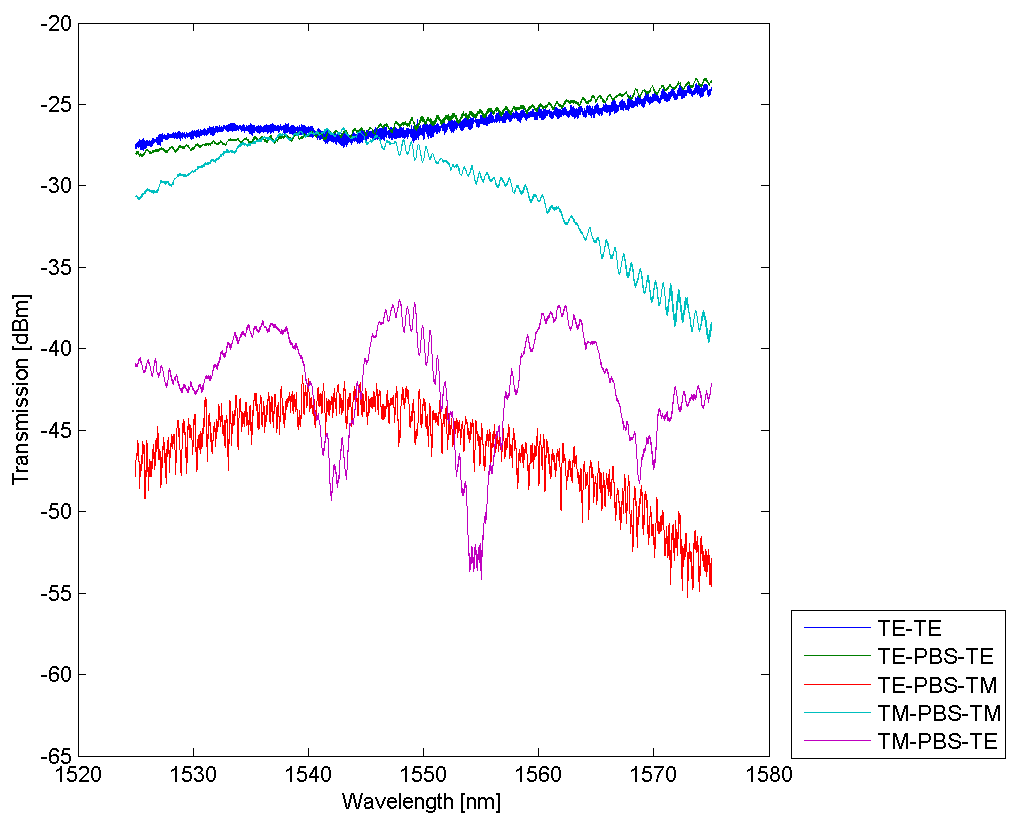
\includegraphics[width=\textwidth]{6-pbs}
		\caption{\gls{pbs} with \gls{te}/\gls{tm} input}
		\label{fig:6_pbs}
	\end{figure}
	
	\subsection{Passive polarization rotator}
	To analyze the data of the \gls{tpr} it is necessary to have a benchmark. Since, the idea of \gls{tpr} is based on canceling the effect of passive \gls{pr} the base measurements of polarization rotation by the \gls{pr} will help to evaluate the results of \gls{tpr}. Since, the cross-section of the stair waveguide is $\chem{160 \times \SI{260}{\nano \meter}}$ the $\chem{L_\pi}$ is calculated accordingly. However, as the modes in the stair waveguide are deconfined, there can be coupling from the evanescent fields. That is why different $\chem{L_\pi}$ lengths are being tried out. In Fig. \ref{fig:6_pr_passive_te}, the graph shows four plots which has \gls{te} input and both \gls{te} and \gls{tm} outputs for different lengths of $\chem{L_\pi}$. The notation $\chem{\gls{te}-\gls{pr}B20-\gls{tm}_{pas}}$ means that the input is \gls{te} and it passes through a passive \gls{pr} of length \SI{20}{\micro \meter} and the output is \gls{tm}. The results in Fig.  \ref{fig:6_pr_passive_te} shows that the passive \gls{pr} is rotating polarization by around \SI{5}{\decibel} after comparing it to Fig. \ref{fig:6_pbs}. In this passive \gls{pr}, the \gls{te} transmission has shifted down by \SI{5}{\decibel} - \SI{10}{\decibel}, whereas, the \gls{tm} transmission has been lifted up by \SI{5}{\decibel} - \SI{10}{\decibel}, which can be seen by comparing Fig. \ref{fig:6_pr_passive_te} and Fig. \ref{fig:6_pbs}.
	
	\begin{figure}[H] %H
		\centering
		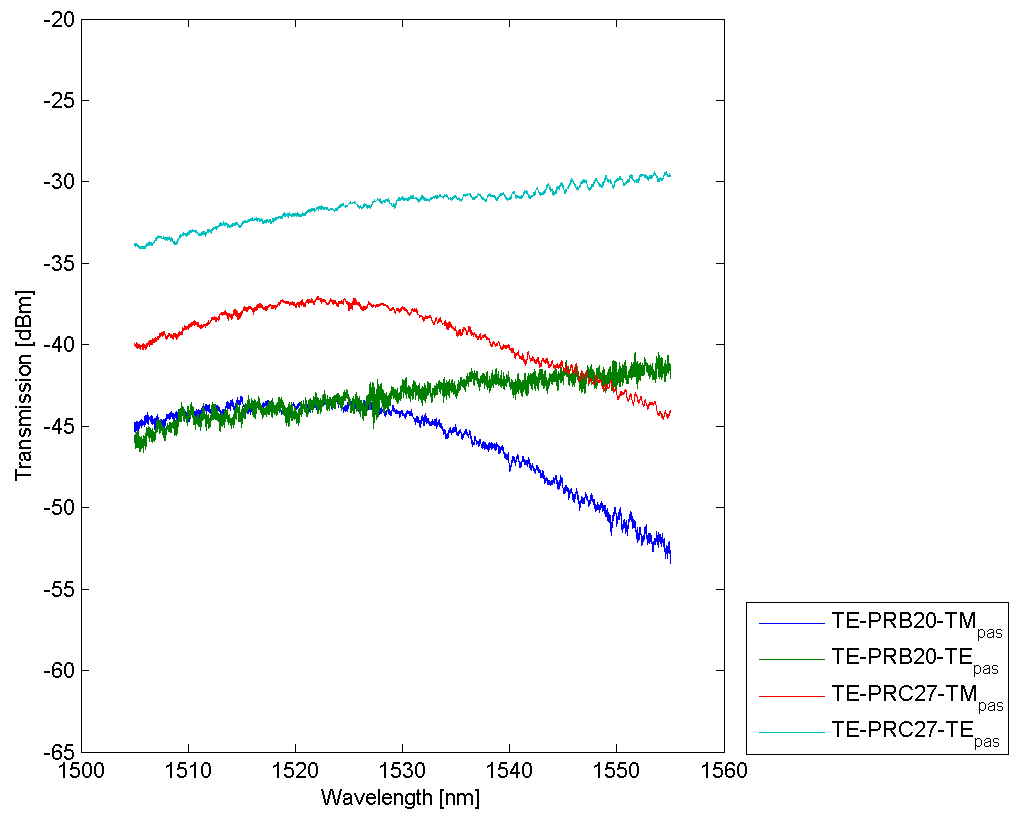
\includegraphics[width=1\textwidth]{6-pr-passive-te}
		\caption{Passive \gls{pr} with \gls{te} input for different cross-section lengths}
		\label{fig:6_pr_passive_te}
	\end{figure}
	
	\subsection{Active polarization rotator}
	To characterize the \gls{tpr}, it is necessary to normalize the results from the results obtained from the \gls{pbs} in \ref{fig:6_pbs}. Also, due to the coupling of the evanescent fields in the deconfined modes, different $\chem{L_\pi}$ lengths are being tried out ($\chem{L_\pi}$ = \SI{25}{\micro \meter}, \SI{20}{\micro \meter}). \par
	As seen in Fig. \ref{fig:6_pr25_active_te}, at \SI{0}{\volt} the \gls{te}-\gls{te} and \gls{te}-\gls{tm} transmission follows the same curve as in \ref{fig:6_pbs}. After applying \SI{4}{\volt}, the \gls{te}-\gls{te} transmission drops by \SI{3}{\decibel} - \SI{5}{\decibel}, whereas, the \gls{te}-\gls{tm} transmission increases by \SI{5}{\decibel} - \SI{10}{\decibel} over \SI{1530}{\nano \meter} - \SI{1575}{\nano \meter} wavelength spectrum. By applying \SI{7}{\volt}, the \gls{te} - \gls{te} transmission decreases even further in the whole spectrum from \SI{1525}{\nano \meter} - \SI{1575}{\nano \meter}, except in \SI{1530}{\nano \meter} - \SI{1545}{\nano \meter},  where the transmission increases by \SI{1}{\decibel} - \SI{2}{\decibel}, which might have occurred due to any abrupt wavelength dependent geometry in the \gls{pr} cross-section. However, by applying \SI{7}{\volt}, the \gls{te} - \gls{tm} transmission increases in the whole spectrum from \SI{1525}{\nano \meter} - \SI{1575}{\nano \meter} as expected. However, when the voltage was tuned off, the \gls{te}-\gls{te} and \gls{te}-\gls{tm} did not come back to their initial state as shown in Fig. \ref{fig:6_pr25_active_tm} (labels: \gls{te}-\gls{pr}25-\gls{te}(0Vback), \gls{te}-\gls{pr}25-\gls{tm}(0Vback)), which suggests that the cantilever might have been collapsed as shown in Fig. \ref{fig:5_tm_sticked_mems}. \par
	\begin{figure}[H] %H
		\centering
		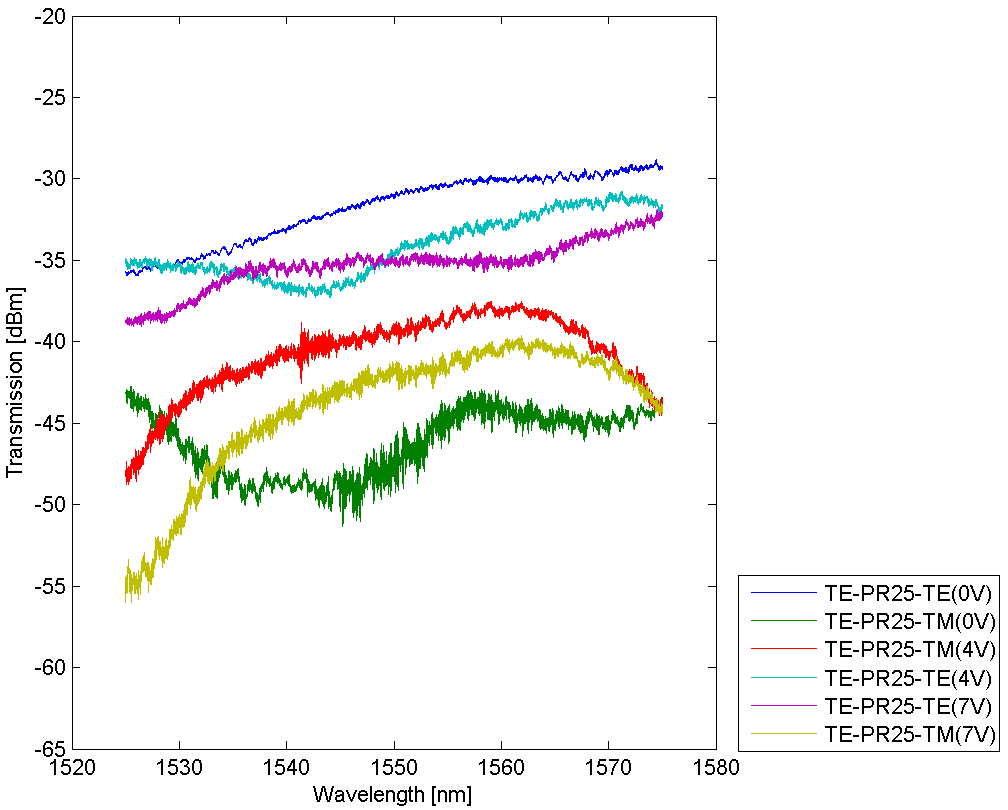
\includegraphics[width=1.0\textwidth]{6-pr25-active-te}
		\caption{\gls{tpr} with \gls{te} input at different voltage inputs for $\chem{L_\pi}$ = \SI{25}{\micro \meter}}
		\label{fig:6_pr25_active_te}
	\end{figure}
	
	\begin{figure}[H] %H
		\centering
		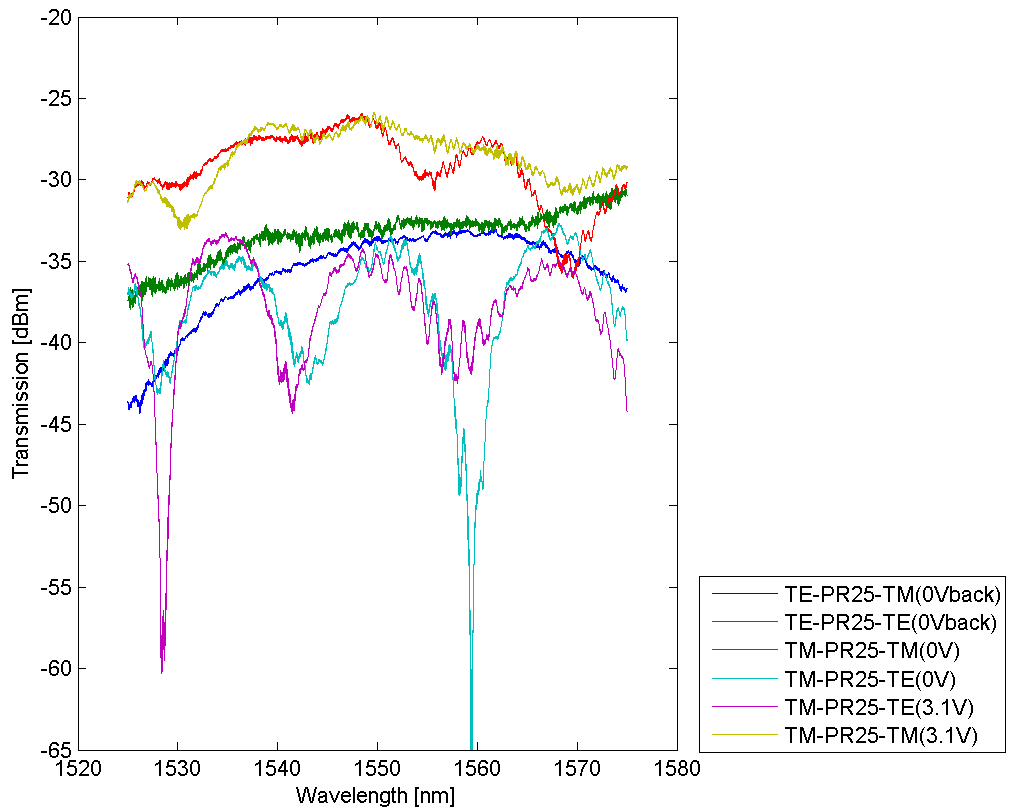
\includegraphics[width=1.0\textwidth]{6-pr25-active-tm}
		\caption{\gls{tpr} with \gls{tm} input at different voltage inputs for $\chem{L_\pi}$ = \SI{25}{\micro \meter}}
		\label{fig:6_pr25_active_tm}
	\end{figure}
	
	The \gls{tm}-\gls{te} \gls{tpr} shown in Fig. \ref{fig:6_pr25_active_tm} does not show any promising results as the \gls{pr} cross-section was not well patterned due to over-exposure during the fabrication which can be seen in Fig. \ref{fig:5_tm_pr_zoom}. Also, there is a interference pattern in the \gls{tm}-\gls{te} transmission which might have arise due to the under-etched cavity in the \gls{tm} gratings and taper. \par
	
	Finally, as shown in Fig. \ref{fig:6_pr20_active_te} the \gls{te}-\gls{tm} \gls{tpr} is analyzed for a cross-section length of \SI{20}{\micro \meter}.
	The results obtained at \SI{0}{\volt} follows the simulation in Fig. \ref{fig:4_stair_s_param_200_230}. When applying \SI{3}{\volt} and \SI{3.4}{\volt} consecutively, the \gls{te} transmission drops by \SI{1}{\decibel} and \SI{6}{\decibel}, whereas, the \gls{tm} transmission increases by \SI{5}{\decibel} and \SI{8}{\decibel} respectively in \SI{1525}{\nano \meter} - \SI{1570}{\nano \meter} wavelength spectrum.
	
	\begin{figure}[H] %H
		\centering
		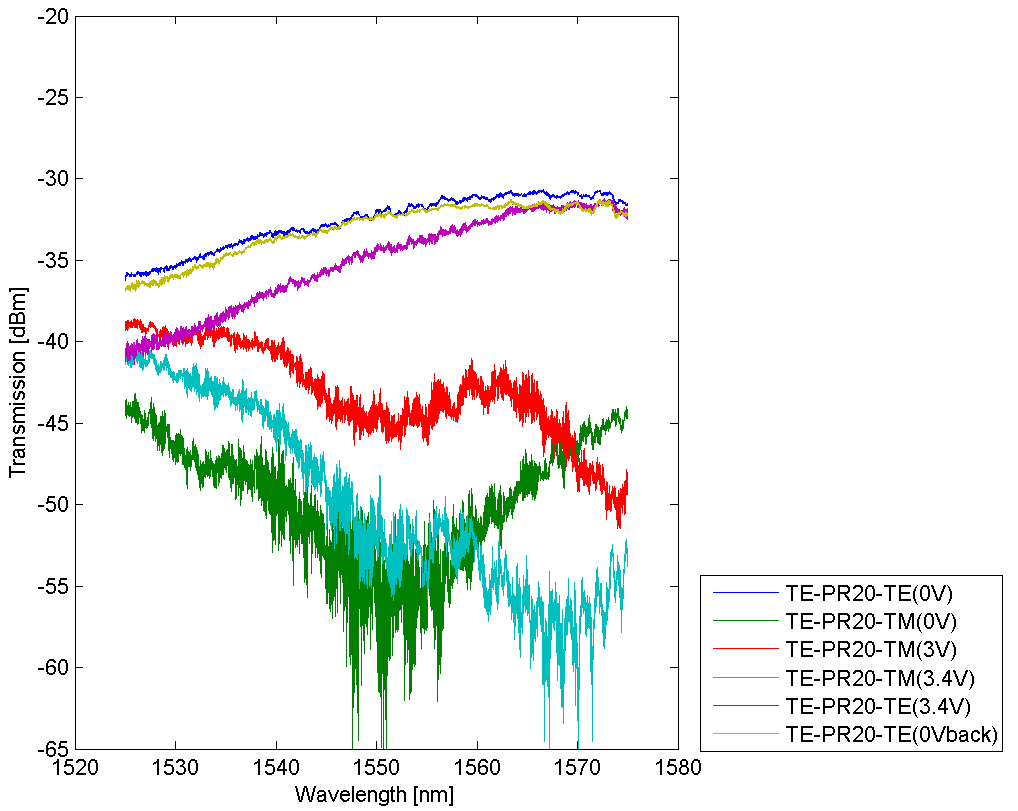
\includegraphics[width=1.0\textwidth]{6-pr20-active-te}
		\caption{\gls{tpr} with \gls{tm} input at different voltage inputs for $\chem{L_\pi}$ = \SI{20}{\micro \meter}}
		\label{fig:6_pr20_active_te}
	\end{figure}
	
	\section{Analysis}
	The results obtained shows that the \gls{pbs} works as intended with \gls{per} $\geq$ \SI{20}{\decibel} in \SI{1525}{\nano \meter} - \SI{1575}{\nano \meter} wavelength spectrum. However, some interference pattern arises in the \gls{tm} transmission as a result of formation of standing waves due to the presence of under-etched cavity in the \gls{tm} gratings and taper. Also, as seen in Fig. \ref{fig:5_tm_pr_zoom}, the stair waveguide cross-section at the beginning of the \gls{pr} is over-exposed in the \gls{tm} input \gls{tpr}. This might also induce reflections in the results obtained, which can create interference. Also, it is difficult to understand from the \gls{sem} the position of the cantilever. For the \gls{tpr} to work, the cantilever must be in same plane or above, than the plane of the suspended bus waveguide. This can happen if the cantilevers are long. So, shorter cantilevers are required to fabricate in plane cantilevers and get promising results. Finally, from the results obtained it can be concluded that the concept of \gls{mems} \gls{tpr} works. Although, much more precise fabrication and characterization is necessary to achieve a high \gls{per} in the C and L bands. The current fabricated \gls{mems} \gls{tpr} with a length of \SI{25}{\micro \meter}, produces a \gls{per} of \SI{5}{\decibel} - \SI{10}{\decibel} in the \SI{1530}{\nano \meter} - \SI{1570}{\nano \meter} wavelength spectrum.
 
\end{document}
